
\section{Evaluation}
\label{sec:evaluation}
%\pgfplotstableread[col sep=comma]{csv-data/average-bandwidth.csv}\tableaverage
%\pgfplotstableread[col sep=comma]{csv-data/average-bandwidth-real-trace.csv}\tableaveragereal
%\pgfplotstableread[col sep=comma]{csv-data/plot-global-time-cdf.csv}\tableglobaltime
%\pgfplotstableread[col sep=comma]{csv-data/plot-local-deltas-cdf.csv}\tablelocaldeltas
%\pgfplotstableread[col sep=comma]{csv-data/plot-local-time-cdf.csv}\tablelocaltime
In this section we present our results. In the following benchmarks \epto uses a constant $c$ to set the probability of a hole appearing. We set $c = 4$ in all our benchmarks so as to not experience any holes as \jgroups does not produce holes under normal conditions. We use a $\delta$ period of \SI{100}{\milli\second} for tests with no churn or synthethic churn and \SI{250}{\milli\second} for tests following a real trace.
\par
We write the cluster parameters as $(n,e)$, where $n$ designates the total number of peers and $e$ denominates the global event throughput per second. We test \epto and \jgroups with three different cluster parameters:
\begin{description}[\IEEEsetlabelwidth{$(100,100)$:}]
	\item[\textbf{$(50,50)$}:] 50 peers with a global event throughput of 50 events per second.
	\item[\textbf{$(50,100)$}:] 50 peers with a global event throughput of 100 events per second.
	\item[\textbf{$(100,50)$}:] 100 peers with a global event throughput of 50 events per second. These parameters are also used for all synthetic churns.
\end{description}
\par 
We use specific settings recommended by \jgroups for a big cluster \autocite{udp-largecluster}.
\par
Every \jgroups test run with churn is run once killing the coordinator and once not killing it. We use the following nomenclature to differentiate both tests:
\begin{description}[\IEEEsetlabelwidth{\jgroups-nocoord: }]
	\item[\textbf{\jgroups-coord}:] The coordinator is killed once.
	\item[\textbf{\jgroups-nocoord}:] The coordinator is purposely kept alive throughout the experiment.
\end{description}
\par
\textbf{Testbed.} \mm{this sentence is not necessary} \jt{I specified it as the following text is really close to the one in Sebastien work as we use the same cluster and I don't want any problem being accused of copy}Our work uses the same cluster first used in \autocite{vaucher2016erasure}. It consists of 20 machines interconnected by a \SI{1}{\gbps} switched network. Each machine has an 8-core Intel Xeon CPU and \SI{8}{\giga\byte} of RAM. We deploy 12 virtual machines on these hosts. Each virtual machine has access 4 VCPUs as well as \SI{7}{\giga\byte} of RAM. We use KVM as our hypervisor. Each VM uses Debian as its O/S. Protocols are packaged as docker images. We use Docker 1.12 and its new functionality Docker Swarm to orchestrate our services. Each docker container has a memory restriction of \SI{300}{\mega\byte} of RAM to be certain we will not have out of memory problems.
\par
\textbf{Experiment parameters.} Every benchmark except the ones following a real trace are run 10 times, each during \SI{20}{\minute}. When there is synthetic churn, the churn starts \SI{30}{\second} after the benchmark and runs for \SI{17}{\minute}. The benchmarks following a real trace are run 5 times. The trace is sped-up 2 times, which means we follow \SI{2}{\hour} worth of trace in \SI{1}{\hour}. Every benchmark run with churn is run with the $(100,50)$ parameters. When we have a global event throughput lower than the number of actual peers, we use a uniform random number generator to artificially reduce the global event throughput. For example, using $(100,50)$ parameters, each peer has a 50\% probability of sending an event at each second.
\par
We compare \epto and \jgroups based on their bandwidth, the local and global time to deliver every expected events, their local dissemination stretch and finally the number of events sent on average.
\subsection{Bandwidth}
The bandwidth metric shows the instantaneous bandwidth, where the bandwidth is the addition of the upload and the download speed.
The initial bandwidth peaks observed for \epto are due to the PSS initialization. When a node starts, it receives an initial view and then quickly runs the PSS active thread four times to jump-start itself.
 \begin{figure}[hpt]
 	\centering
 	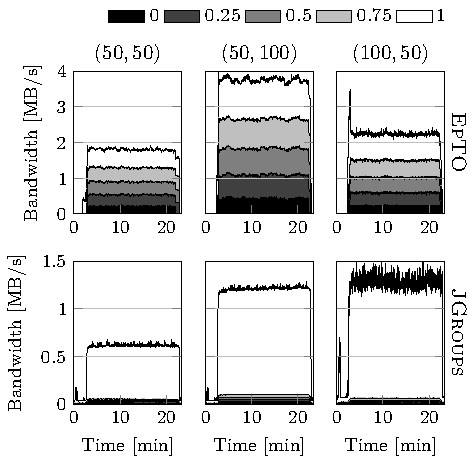
\includegraphics[width=\linewidth]{figures/bandwidth-nochurn.pdf}
 	\vspace{-2mm} 
 	\caption{Bandwidth percentiles of nodes during a stable experiment}
 	\vspace{-2mm} 
 	\label{fig:bandwidth}
 \end{figure}
In \autoref{fig:bandwidth} we observe that \epto has a worse baseline compared to \jgroups. It uses a median bandwidth of approximately \SI{1}{\mbps} for $(50,50)$ whereas \jgroups uses a median bandwidth of less than \SI{0.2}{\mbps}. However, in \jgroups most of the work is done solely by the coordinator. We can clearly see this as the 100th percentile is much higher than the rest and uses approximately \SI{.6}{\mbps}.

Comparing \epto and \jgroups in terms of bandwidth when we increase the number of events sent per second, we can see the bandwidth doubling in both cases. In lower peers scenario such as the ones presented in \autoref{fig:bandwidth} \jgroups is clearly at an advantage. Since \epto has a worse baseline we will reach the maximum bandwidth available much quicker when increasing the event throughput.

Comparing \epto and \jgroups in terms of bandwidth when we increase the number of peers, \epto scales better than \jgroups. While \jgroups basically has to double the bandwidth usage of the coordinator, \epto only increases it marginally. Thus in a scenario where we have many peers \epto will be more efficient than \jgroups at not reaching the maximum available bandwidth on a given node.\mm{it would be perfect if we could experimentally show this.}
 \begin{figure}[hpt]
 	\centering
 	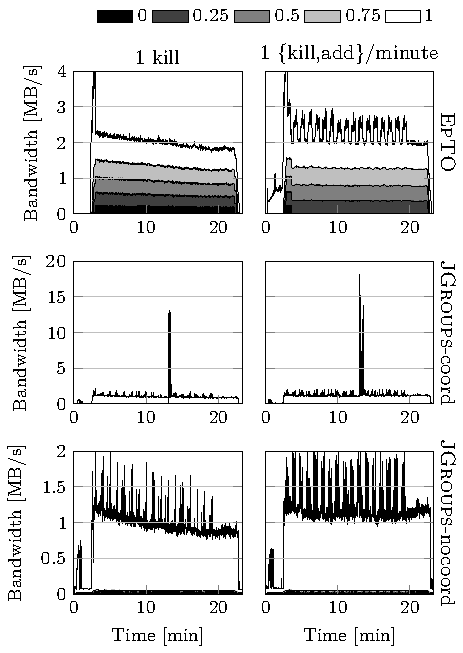
\includegraphics[width=\linewidth]{figures/bandwidth-synth-churn.pdf}
 	\vspace{-2mm} 
 	\caption{Bandwidth percentiles of nodes during an unstable experiment with synthetic churn}
 	\vspace{-2mm} 
 	\label{fig:bandwidth-churn}
 \end{figure}
\par
In \autoref{fig:bandwidth-churn} we analyze two different synthetic churns. In the first one we kill one node per minute. In the second one, we still kill one node per minute, but we immediately create a new one. For \jgroups we run the benchmarks once without killing the coordinator and once killing it.

We can see that the churn does not affect \epto at all when there are only nodes leaving. We have small peaks when adding a node to \SI{3}{\mbps} or less which can be explained by the PSS initialization. This is confirmed at the end of the plot where \epto goes back to a normal Bandwidth after stabilization.

On the other hand, when killing the coordinator in \jgroups we can see a huge spike in bandwidth, going from \SI{1.2}{\mbps} to more than \SI{15}{\mbps}. This is due to how \jgroups operates when selecting a new coordinator which requires detecting the coordinator failure, electing a new coordinator and propagating these changes.

Even when not killing the coordinator, \jgroups suffers from the churn. We can see that each time the view changes, it generates an almost 100\% increase in bandwidth usage. This is due to \jgroups having to update the view and propagate it to every peer.

These results are quite interesting as they confirm two common held beliefs in the community: deterministic protocols behave pooly under churn, and probabilistic protocols are largely unaffected by churn.

\subsection{Total GigaBytes sent/received}
This metric shows the Total number of bytes sent and received on average during an experiment.
In all cases, \jgroups receives more bytes than it sends. This is due to the fact that we do not measure the bandwidth on the TCPGOSSIP, which is in charge of view changes. Thus, when a new peer joins the cluster, the TCPGOSSIP will send a new view to every peer already in the cluster.
\par
\begin{table}[hpt]
	\centering
	\caption{Total \si{\giga\byte} sent/received in a stable system}
	\sisetup{table-format=2.2, separate-uncertainty, table-figures-uncertainty = 2, table-align-uncertainty}
	\resizebox{\linewidth}{!}{
	\begin{tabular}{llSSS}
		\toprule
		&& \multicolumn{3}{c}{Cluster parameters} \\
		\cmidrule{3-5}
		{Protocol}&& {$(50,50)$} & {$(50,100)$} & {$(100,50)$} \\
		\midrule
		\multirow{2}{*}{\epto}&{Receive}& 10.84(016) & 22.31(039) & 26.01(027) \\
						    &{Sending}& 10.84(016) & 22.31(039) & 26.01(027)\\
		\midrule
		\multirow{2}{*}{\jgroups}&{Receive}& 0.78(003) & 1.45(001) & 1.88(001)\\
							   &{Sending}& 0.77(003) & 1.44(001) & 1.84(001)\\
		\bottomrule
	\end{tabular}
	}
	\label{table:total-bandwidth} 
\end{table}
In \autoref{table:total-bandwidth}, \epto has a worse baseline than \jgroups. This is expected as \epto sends $c*n*\log_2 n$ messages per events and \jgroups sends at least $n$ messages per event so we should have at least $c*\log_2 n$ more messages sent in \epto if \jgroups is perfect. Here we are well within this ratio.
\begin{table}[hpt]
	\centering
	\caption{Total \si{\giga\byte} sent/received with a synthetic churn}
	\sisetup{table-format=2.2, separate-uncertainty, table-figures-uncertainty = 2, table-align-uncertainty}
	\resizebox{\linewidth}{!}{
	\begin{tabular}{lSSS}
		\toprule
		&& \multicolumn{2}{c}{Churn parameters} \\
		\cmidrule{3-4}
		{Protocol}&& {1 kill/minute} & {1\{kill,add\}/minute} \\
		\midrule
		\multirow{2}{*}{\epto}&{Receive}& 21.00(024) & 26.32(032)\\
							&{Sending}& 21.21(025) & 26.57(032)\\
		\midrule
		\multirow{2}{*}{\jgroups-coord}&{Receive}& 1.47(002) & 1.75(002)\\&{Sending}& 1.43(002) & 1.70(002)\\
		\midrule
		\multirow{2}{*}{\jgroups-nocoord}&{Receive}& 1.45(001) & 1.73(002)\\&{Sending}& 1.41(001) & 1.68(002)\\
		\bottomrule
	\end{tabular}
	}
	\label{table:total-bandwidth-churn} 
\end{table}
In \autoref{table:total-bandwidth-churn} we see that \jgroups total bandwidth usage is smaller when there is churn. One hypothesis for this is that a \jgroups replica takes a longer time to start up compared to stopping a replica. Therefore the overall benchmark has a longer time with less than 100 replicas. We also do not see a difference whether we kill the coordinator or not. This can be explained by the fact that before the detection of a faulty coordinator \jgroups is forced to a halt for period of up to \SI{20}{\second} making the system unavailable. 
\subsection{Local Times}
\label{sub:local-times}
The local time represents the total time it takes for a peer to deliver every \mm{missing text}.
 \begin{figure*}[hpt]
 	\centering
 	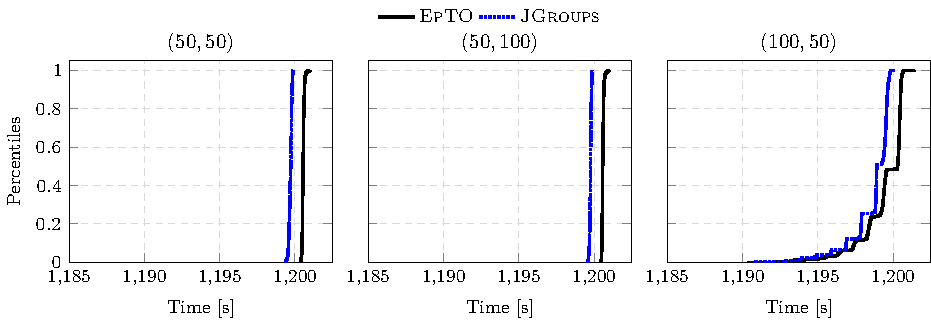
\includegraphics[width=\linewidth]{figures/local-times-nochurn.pdf}
 	\vspace{-2mm} 
 	\caption{Local dissemination times}
 	\vspace{-2mm}
 	\label{fig:local-times} 
 \end{figure*}

 \begin{figure}[hpt]
 	\centering
 	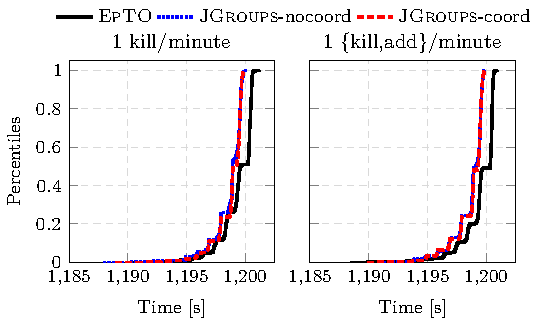
\includegraphics[width=\linewidth]{figures/local-times-synth-churn.pdf}
 	\vspace{-2mm} 
 	\caption{Local dissemination times with churn}
 	\vspace{-2mm} 
 	\label{fig:local-times-churn} 
 \end{figure}
In \autoref{fig:local-times}, \jgroups delivers all events quicker than \epto in all scenarios, even when churn is involved as is shown in \autoref{fig:local-times-churn}. However, \epto is not too far behind. The difference between \epto and \jgroups is likely to be even smaller when running them in a real WAN network due to the latency. \epto in our configuration has a $\delta$ period of \SI{100}{\milli\second} and is thus handicapped against \jgroups in a LAN environment, because it only increments the TTL of an event every \SI{100}{\milli\second}. We expect \epto to outperform \jgroups in this situation when we have a high number of peers in the system or when the network has a higher latency. Furthermore, in our test environment \jgroups is not limited by the bandwidth. If the coordinator would have a lower limit of bandwidth, the time to send all events when the coordinator dies would be longer.\mm{we could try to setup an AWS test in mutliple availability zones to see what happens.} \jt{Yes I though about it too. Unfortunately we can't make it work for the moment :/}
\subsection{Global Times}
The global time represents the total time it takes for all peers to deliver every event sent.\mm{this is imprecise, review. same for local time}
 \begin{figure*}[hpt]
 	\centering
 	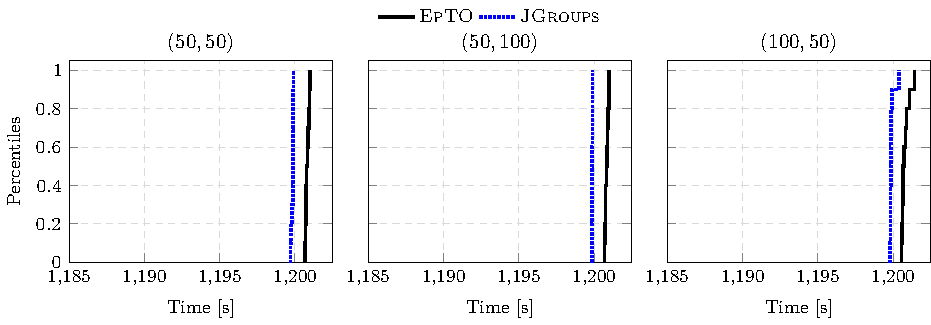
\includegraphics[width=\linewidth]{figures/global-times-nochurn.pdf}
 	\vspace{-2mm} 
 	\caption{Global dissemination times}
 	\vspace{-2mm}
 	\label{fig:global-times}  
 \end{figure*}

 \begin{figure}[hpt]
 	\centering
 	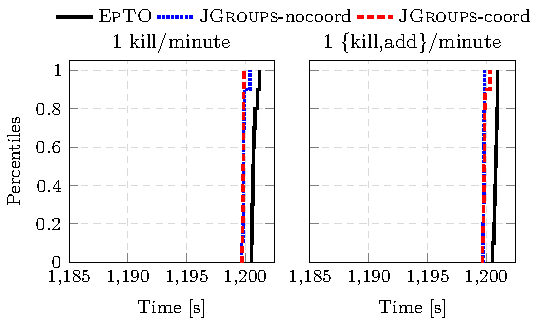
\includegraphics[width=\linewidth]{figures/global-times-synth-churn.pdf}
 	\vspace{-2mm} 
 	\caption{Global dissemination times with churn}
 	\vspace{-2mm} 
 	\label{fig:global-times-churn} 
 \end{figure}
Global times are represented in \autoref{fig:global-times} and \autoref{fig:global-times-churn}. These global times are of less interest than their local counterpart as the differences in clocks between hosts can skew this measurement.
\mm{explain why the fact that the system system stops for about 20 seconds when the coordinator dies is not observable in these measurements. }

Nonetheless, here too we can see that \epto is consistently slower than \jgroups for the same reason as stated in \autoref{sub:local-times}.
\subsection{Local Dissemination stretch}
The local dissemination stretch is the time measurement between the sending of an event by a peer and the delivery of this event locally.
 \begin{figure}[hpt]
 	\centering
 	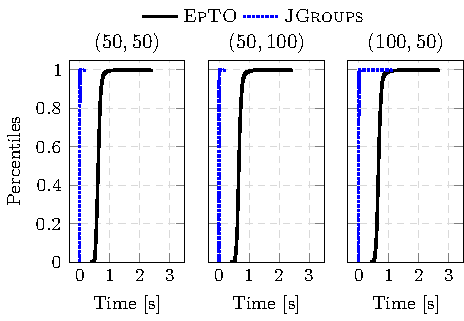
\includegraphics[width=\linewidth]{figures/local-diss-stretch-nochurn.pdf}
 	\vspace{-2mm} 
 	\caption{Local dissemination stretch}
 	\vspace{-2mm}
 	\label{fig:local-delta}  
 \end{figure}
In \autoref{fig:local-delta}, we see the percentiles of the local dissemination stretch.
\par
\jgroups is usually much faster than \epto in a perfect environment. This is expected as the benchmarks involve a small number of nodes and are performed in a LAN environment with minimal latency. The median dissemination stretch of \jgroups is around \SI{7}{\milli\second} where as the median dissemination stretch of \epto is around \SI{630}{\milli\second} for $(100,50)$. When increasing the number of peers, \jgroups starts to have longer delivery times for some outliers. A small portion of the local dissemination stretches are really fast (\SI{1}{\milli\second} or lower). This happens when the coordinator itself sends an event. Since it has to deliver it to himself the local dissemination stretch is intra-process and thus extremely fast.

 \begin{figure}[hpt]
 	\centering
 	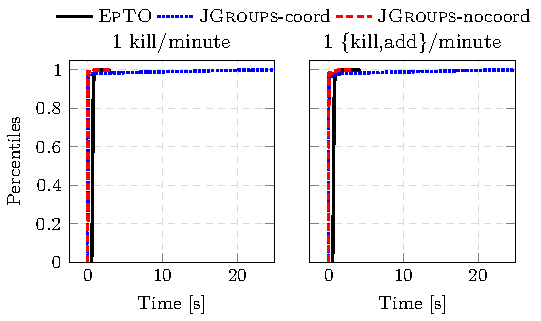
\includegraphics[width=\linewidth]{figures/local-diss-stretch-synth-churn.pdf}
 	\vspace{-2mm} 
 	\caption{Local dissemination stretch with churn}
 	\vspace{-2mm}
 	\label{fig:local-delta-churn}   
 \end{figure}
In \autoref{fig:local-delta-churn} We see a completely different picture. When under churn, the 95th percentile of \jgroups is at \SI{31}{\milli\second} compared to \SI{14}{\milli\second} when there is no churn. The highest percentiles are at more than \SI{20}{\second}. This effect is due to the coordinator dying as we clearly see that it does not happen when we do not kill it.

The median is bigger at around \SI{9}{\milli\second}, whether we kill the coordinator or not. This shows that there are some degradation in \jgroups local dissemination stretch when under churn.

On the contrary, \epto performs very well under churn. The median degrades a bit at \SI{650}{\milli\second} with the 99th percentile being at \SI{1030}{\milli\second} compared to \SI{982}{\milli\second} when no churn is happening.
\subsection{Events sent}
\mm{explain first what this is before pointing out what was observed.}
The variation observed in the different tests are due to the fact that we use \textit{Thread.sleep()} between each send and that in some configurations a randomness decides whether an event is sent or not.
\begin{table}[hpt]
	\centering
	\caption{Total events sent in a stable environment}
\sisetup{table-format=6.1, separate-uncertainty, table-figures-uncertainty = 2, table-align-uncertainty}
\begin{tabular}{lSSS}
	\toprule
	& \multicolumn{3}{c}{Cluster parameters} \\
	\cmidrule{2-4}
	Protocol & {$(50,50)$} & {$(50,100)$} & {$(100,50)$} \\
	\midrule
	\epto & 59993.8(33) & 119898.2(97) & 59913.0(1643) \\
	\jgroups & 59961.9(109) & 119885.7(50) & 60023.1(2871) \\
	\bottomrule
\end{tabular}
\label{table:total-events}  
\end{table}

In \autoref{table:total-events} we see that both \epto and \jgroups deliver the same amount of events. This is expected in a perfect environment.
\begin{table}[hpt]
	\centering
	\caption{Total events sent with a synthetic churn}
\sisetup{table-format=6.1, separate-uncertainty, table-figures-uncertainty = 2, table-align-uncertainty}
\begin{tabular}{lSSS}
	\toprule
	& \multicolumn{2}{c}{Cluster parameters} \\
	\cmidrule{2-3}
	Protocol & {1 kill/minute} & {1\{kill,add\}/minute} \\
	\midrule
	\epto & 53898.5(1339) & 59798.6(1401) \\
	\jgroups-coord & 53834.7(1755) & 59507.9(2409) \\
	\jgroups-nocoord & 53830.5(2003) & 59450.5(1751) \\
	\bottomrule
\end{tabular}
    \label{table:total-events-churn}
\end{table}
In \autoref{table:total-events-churn} When only killing nodes, \epto and \jgroups again deliver the same amount of events. When killing and adding nodes, \jgroups delivers a smaller amount of events.
This is explained by the fact that \jgroups nodes take longer to start but the differences do not look significant enough to draw any conclusion. \jt{I didn't run any statistical analysis}
\subsection{Real Trace}
 \begin{figure}[hpt]
 	\centering
 	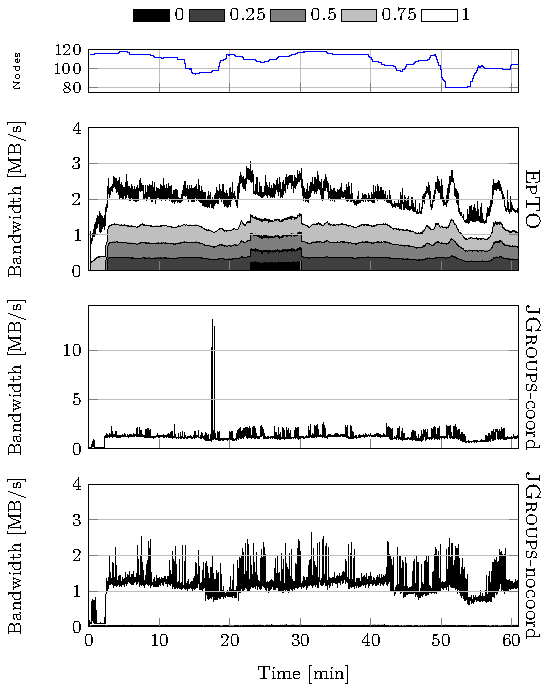
\includegraphics[width=\linewidth]{figures/bandwidth-real-churn.pdf}
 	\vspace{-2mm} 
 	\caption{Bandwidth percentiles of a node during an experiment with a real churn}
 	\vspace{-2mm} 
 	\label{fig:bandwidth-real-churn}
 \end{figure}
\autoref{fig:bandwidth-real-churn} confirms the results from the synthetic churn. \epto is not affected by the churn. As before, \jgroups is affected in the same situations as when following a synthetic churn. The spikes visible on \jgroups-coord and \jgroups-nocoord show the different view changes occuring. 
\par
\begin{table}[hpt]
	\centering
	\caption{Total \si{\giga\byte} sent/received}
	\sisetup{table-format=2.2, separate-uncertainty, table-figures-uncertainty = 2, table-align-uncertainty}
	\begin{tabular}{lSS}
		\toprule
		&& \multicolumn{1}{c}{Churn parameters} \\
		\cmidrule{3-3}
		{Protocol}&& {Real Trace} \\
		\midrule
		\multirow{2}{*}{\epto}&{Receive}& 81.41(108)\\
		&{Sending}& 82.67(108)\\
		\midrule
		\multirow{2}{*}{\jgroups-coord}&{Receive}& 5.56(008)\\
		&{Sending}& 5.40(008)\\
		\midrule
		\multirow{2}{*}{\jgroups-nocoord}&{Receive}& 5.58(005)\\
		&{Sending}& 5.43(005)\\
		\bottomrule
	\end{tabular}
	\label{table:total-bandwidth-real-churn} 
\end{table}
\autoref{table:total-bandwidth-real-churn} also confirms our earlier results. \epto is still within the $c*log_2(n)$ ratio fixed earlier.
\par
\begin{figure}[hpt]
	\centering
	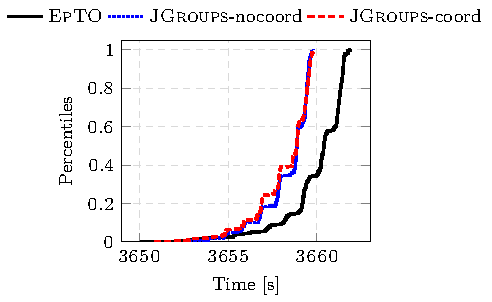
\includegraphics[width=\linewidth]{figures/local-times-real-churn.pdf}
	\vspace{-2mm} 
	\caption{Local dissemination times}
	\vspace{-2mm}
	\label{fig:local-times-real-churn} 
\end{figure}
\begin{figure}[hpt]
	\centering
	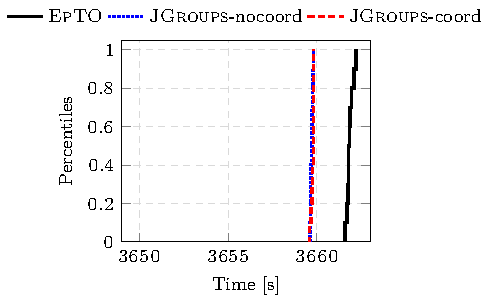
\includegraphics[width=\linewidth]{figures/global-times-real-churn.pdf}
	\vspace{-2mm} 
	\caption{Global dissemination times with a real churn}
	\vspace{-2mm} 
	\label{fig:global-times-real-churn} 
\end{figure}
The local and global dissemination times shown in respectively \autoref{fig:local-times-real-churn} and \autoref{fig:global-times-real-churn} still show \jgroups to outperform \epto in this scenario. Again, we want to emphasize that it is expected for \jgroups to perform better than \epto with the cluster size we use.
\par
\begin{figure}[hpt]
	\centering
	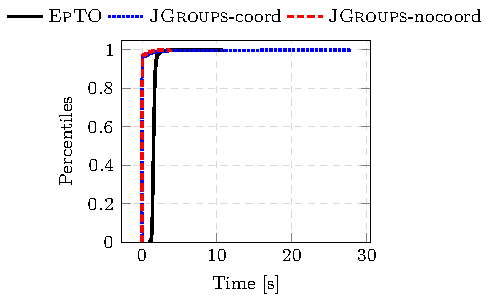
\includegraphics[width=\linewidth]{figures/local-diss-stretch-real-churn.pdf}
	\vspace{-2mm} 
	\caption{Local dissemination stretch with a real churn}
	\vspace{-2mm}
	\label{fig:local-delta-real-churn}   
\end{figure}
In \autoref{fig:local-delta-real-churn}, \epto has worse outliers than before and so does \jgroups-coord.
\begin{table}[hpt]
	\centering
	\caption{Total events sent during a real trace}
\sisetup{table-format=6.1, separate-uncertainty, table-figures-uncertainty = 6, table-align-uncertainty}
\begin{tabular}{lS}
	\toprule
	Protocol & {Events sent}\\
	\midrule
	\epto & 165844.2(2102)\\
	\jgroups-coord & 166183.0(13681)\\
	\jgroups-nocoord & 166585.8(8249)\\
	\bottomrule
\end{tabular}
    \label{table:total-sent-real-churn}
\end{table}
\autoref{table:total-bandwidth-real-churn} is interesting. We see that on average \jgroups seems to deliver more events than \epto, but its standard deviation is way higher than that of \epto, suggesting \epto to be more stable and consistent.
\subsection{Problems encountered}
When running \jgroups we sometimes get failed runs, where either some peers will experience holes or a peer will deliver out of order events. These failed runs only happen when there is churn happening, specifically when we add and remove peers and when the coordinator dies. These problems appeared 3 times out of 13 runs for \jgroups $1\{kill,add\}/minute$ and 2 times out of 7 for \jgroups with real churn. We have not investigated these problems further. This points to either \jgroups failing when there is too much churn or a bug present in the SEQUENCER implementation.

We measure holes as one or more events that were delivered by at least one peer in the cluster but not on the peer containing the hole. As stated earlier, we specifically choose a $c$ high enough to never experience holes in \epto as \jgroups should never suffer from holes. If either \jgroups or \epto fails to deliver every event sent during the run, the run is considered as having a problem.
